\documentclass{standalone}
\usepackage{xcolor}
\usepackage{tikz}
\usepackage{pgfplots}
\pgfplotsset{compat=1.18}
\definecolor{original}{HTML}{d5002d}
\definecolor{simple}{HTML}{03af7a}
\definecolor{approx}{HTML}{005aff}
\begin{document}
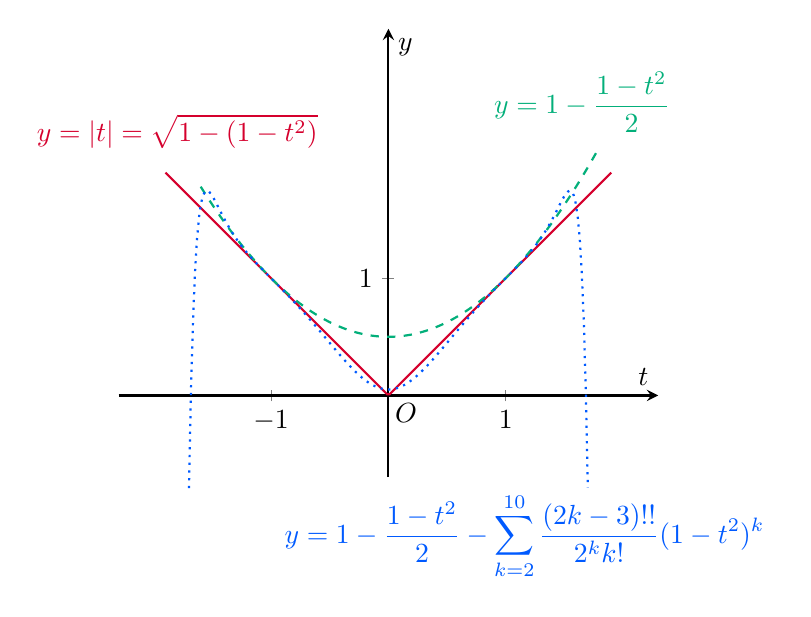
\begin{tikzpicture}
    \begin{axis}[
        axis equal,
        axis lines=middle,
        axis line style=thick,
        xlabel={$t$},
        ylabel={$y$},
        ytick={1},
        yticklabels={$1$},
        xtick={-1, 1},
        xticklabels={$-1$, $1$,},
        domain=-2.5:2.5,
        xmin=-2.3,
        xmax=2.3,
        ymin=-0.07,
        ymax=2.5,
        samples=200,
        clip=false
    ]
        \addplot[original, thick][domain=-1.9:1.9] {abs(x)};
        \addplot[simple, thick, dashed][domain=-1.6:1.77] {1 - (1 - x^2)/2};
        \addplot[approx, thick, dotted][domain=-1.7:1.7] {%
            1
            - (1 - x^2)/2
            - (1 - x^2)^2 / 8
            - 3 * (1 - x^2)^3 / 16
            - 5 * (1 - x^2)^4 / 128
            - 7 * (1 - x^2)^5 / 256
            - 21 * (1 - x^2)^6 / 1024
            - 33 * (1 - x^2)^7 / 2048
            - 429 * (1 - x^2)^8 / 32768
            - 715 * (1 - x^2)^9 / 65536
            - 2431 * (1 - x^2)^10 / 262144
            % - 4199 * (1 - x^2)^11 / 524288
            % - 29393 * (1 - x^2)^12 / 4194304
        };
        \node (O) at (axis cs:0.15, -0.15) {$O$};
        \node (original) at (axis cs:-1.8, 2.25) {%
            \textcolor{original}{$\displaystyle y = |t| = \sqrt{1 - (1 - t^2)}$}
        };
        \node (curve) at (axis cs:1.65, 2.5) {\textcolor{simple}{%
            $\displaystyle y = 1 - \frac{1 - t^2}{2}$}
        };
        \node (lim) at (axis cs:1.2, -1.2) {%
            \textcolor{approx}{%
                $\displaystyle y = 1 - \frac{1 - t^2}{2} - \sum_{k = 2}^{10} \frac{(2k - 3)!!}{2^k k!} (1 - t^2)^k$
            }
        };
    \end{axis}
\end{tikzpicture}
\end{document}
